\documentclass{beamer}
\usepackage[utf8]{inputenc}

\usetheme{Madrid}
\usecolortheme{default}
\usepackage{amsmath,amssymb,amsfonts,amsthm}
\usepackage{txfonts}
\usepackage{tkz-euclide}
\usepackage{listings}
\usepackage{adjustbox}
\usepackage{array}
\usepackage{tabularx}
\usepackage{gvv}
\usepackage{lmodern}
\usepackage{circuitikz}
\usepackage{tikz}
\usepackage{graphicx}

\setbeamertemplate{page number in head/foot}[totalframenumber]

\usepackage{tcolorbox}
\tcbuselibrary{minted,breakable,xparse,skins}



\definecolor{bg}{gray}{0.95}
\DeclareTCBListing{mintedbox}{O{}m!O{}}{%
	breakable=true,
	listing engine=minted,
	listing only,
	minted language=#2,
	minted style=default,
	minted options={%
		linenos,
		gobble=0,
		breaklines=true,
		breakafter=,,
		fontsize=\small,
		numbersep=8pt,
		#1},
	boxsep=0pt,
	left skip=0pt,
	right skip=0pt,
	left=25pt,
	right=0pt,
	top=3pt,
	bottom=3pt,
	arc=5pt,
	leftrule=0pt,
	rightrule=0pt,
	bottomrule=2pt,
	toprule=2pt,
	colback=bg,
	colframe=orange!70,
	enhanced,
	overlay={%
		\begin{tcbclipinterior}
			\fill[orange!20!white] (frame.south west) rectangle ([xshift=20pt]frame.north west);
	\end{tcbclipinterior}},
	#3,
}
\lstset{
	language=C,
	basicstyle=\ttfamily\small,
	keywordstyle=\color{blue},
	stringstyle=\color{orange},
	commentstyle=\color{green!60!black},
	numbers=left,
	numberstyle=\tiny\color{gray},
	breaklines=true,
	showstringspaces=false,
}
%------------------------------------------------------------
%This block of code defines the information to appear in the
%Title page
\title %optional
{2.8.24}

%\subtitle{A short story}

\author % (optional)
{Nipun Dasari - EE25BTECH11042}



\begin{document}
	
	\frame{\titlepage}
	\begin{frame}{Question}
		The $\vec{a} + \vec{b}$ bisects the angle between $\vec{a}$ and $\vec{b}$ if \underline{\hspace{2cm}}
	\end{frame}
	
	
	\begin{frame}{Theoretical Solution}
			Theorem: The $\vec{a} + \vec{b}$ bisects the angle between $\vec{a}$ and $\vec{b}$ if and only if $\norm{\vec{a}}$ = $\norm{\vec{b}}$ \\
		We prove the above in two parts:\\
		Assume a $\vec{c}$ such that
		\begin{align}
			\vec{c} = \vec{a} + \vec{b} \label{0.2}
		\end{align}
		Let $\alpha$ and $\beta$ be angles made by $\vec{c}$ with $\vec{a}$ and $\vec{b}$ respectively.
		\textbf{Part 1}
		Given : 
		\begin{align}
			\norm{\vec{a}} = \norm{\vec{b}} \label{0.1}
		\end{align}
	\end{frame}
	\begin{frame}{Theoretical Solution}
		To prove : $\vec{a} + \vec{b}$ bisects the angle between $\vec{a}$ and $\vec{b}$\\
		Proof: \\	
		The angle $\theta$ between $\vec{p}$ and $\vec{q}$ is given by: 
		\begin{align}
			\cos\theta = \frac{\vec{p}^\top\vec{q}}{\norm{\vec{p}}\norm{\vec{q}}} \label{0.3}
		\end{align}
		By \eqref{0.3} and \eqref{0.2}
		\begin{align}
			\implies \cos\alpha = \frac{\vec{a}^\top\brak{\vec{a}+\vec{b}}}{\norm{\vec{a}}\norm{\vec{a}+\vec{b}}} 
		\end{align}
		\begin{align}
			\implies \cos\beta = \frac{\vec{b}^\top\brak{\vec{a}+\vec{b}}}{\norm{\vec{b}}\norm{\vec{a}+\vec{b}}} 
		\end{align}
	\end{frame}
	
	\begin{frame}{Theoretical Solution}
		By \eqref{0.1}
	\begin{align}
		\vec{a}^\top\vec{a} = \vec{b}^\top\vec{b}
	\end{align}
	\begin{align}
		\vec{a}^\top\vec{a} + \vec{a}^\top\vec{b} = \vec{b}^\top\vec{b} + \vec{b}^\top\vec{a}
	\end{align}
	\begin{align}
		\frac{\vec{a}^\top\vec{a} + \vec{a}^\top\vec{b}}{\norm{\vec{a}}\norm{\vec{a}+\vec{b}}} = \frac{\vec{b}^\top\vec{b} + \vec{b}^\top\vec{a}}{\norm{\vec{b}}\norm{\vec{a}+\vec{b}}}
	\end{align}
	\begin{align}
		\therefore \cos\alpha=	\cos\beta   \label{angle}
	\end{align}	
	\begin{align}
		\therefore	\alpha=\beta
	\end{align}	
	\end{frame}
	\begin{frame}{Theoretical Solution}
			\textbf{Part 2}\\
		\textbf{Part 2}\\
	Given:
	\begin{align}
		\alpha=\beta
	\end{align}
	To prove:
	\begin{align}
		\norm{\vec{a}} = \norm{\vec{b}} 
	\end{align}
	Proof:\\
	By \eqref{angle}
	\begin{align}
		\cos{\alpha}=\cos{\beta}
	\end{align}
	\begin{align}
		\frac{\vec{a}^\top\brak{\vec{a}+\vec{b}}}{\norm{\vec{a}}\norm{\vec{a}+\vec{b}}} = \frac{\vec{b}^\top\brak{\vec{a}+\vec{b}}}{\norm{\vec{b}}\norm{\vec{a}+\vec{b}}}
	\end{align}
	\begin{align}
		\norm{\vec{b}} (\norm{\vec{a}}^2 + \vec{a}^\top\vec{b}) = \norm{\vec{a}} (\norm{\vec{b}}^2 + \vec{a}^\top\vec{b}) \\
		\norm{\vec{b}}\norm{\vec{a}}^2 + \norm{\vec{b}}(\vec{a}^\top\vec{b}) = \norm{\vec{a}}\norm{\vec{b}}^2 + \norm{\vec{a}}(\vec{a}^\top\vec{b})
	\end{align}
	\end{frame}
	\begin{frame}{Theoretical Solution}
		Rearrange the terms to group common factors:
		\begin{align}
			\norm{\vec{b}}\norm{\vec{a}}^2 - \norm{\vec{a}}\norm{\vec{b}}^2 = \norm{\vec{a}}(\vec{a}^\top\vec{b}) - \norm{\vec{b}}(\vec{a}^\top\vec{b})
		\end{align}
		\begin{align}
			\norm{\vec{a}}\norm{\vec{b}} (\norm{\vec{a}} - \norm{\vec{b}}) = (\vec{a}^\top\vec{b}) (\norm{\vec{a}} - \norm{\vec{b}})
		\end{align}
		
		\begin{align}
			(\norm{\vec{a}} - \norm{\vec{b}}) (\norm{\vec{a}}\norm{\vec{b}} - \vec{a}^\top\vec{b}) = 0
		\end{align}
		
	\end{frame}
	\begin{frame}{Theoretical Solution}
		This equation gives two possibilities:
		\begin{align}
			\norm{\vec{a}} - \norm{\vec{b}} = 0 \implies \norm{\vec{a}} = \norm{\vec{b}}\\
			\norm{\vec{a}}\norm{\vec{b}} - \vec{a}^\top\vec{b} = 0 \implies \vec{a}^\top\vec{b} = \norm{\vec{a}}\norm{\vec{b}}\text{} \label{np}
		\end{align}
		\eqref{np} is incorrect as parallel vectors are not being assumed.\\
		Thus proved
	\end{frame}
	\begin{frame}[fragile]
		\frametitle{C Code }
		
		\begin{lstlisting}
		#include <math.h> // Required for sqrt() and fabs()
		
		// Define a small constant for floating-point comparisons
		#define EPSILON 1e-9
		
		// Structure to represent a 3D vector
		typedef struct {
			double x;
			double y;
			double z;
		} Vector3D;
		
		/**
		* @brief Calculates the magnitude (length) of a 3D vector.
		* @param v The input Vector3D.
		* @return The magnitude of the vector.
		*/
			\end{lstlisting}
		\end{frame}
		\begin{frame}[fragile]
			\frametitle{C Code }
			
			\begin{lstlisting}
				double vector_magnitude(Vector3D v) {
					return sqrt(v.x * v.x + v.y * v.y + v.z * v.z);
				}
				
				
				
			\end{lstlisting}
		\end{frame}
		\begin{frame}[fragile]
			\frametitle{C Code}
			
			\begin{lstlisting}
	int does_sum_bisect_angle(Vector3D a, Vector3D b) {
	double mag_a = vector_magnitude(a);
	double mag_b = vector_magnitude(b);
				
// Compare magnitudes with a small tolerance for floating-point numbers.
// If the absolute difference is less than EPSILON, consider them equal.
if (fabs(mag_a - mag_b) < EPSILON) {
return 1; // Magnitudes are approximately equal.
} else {
return 0; // Magnitudes are not equal.
				
			\end{lstlisting}
		\end{frame}
		
		\begin{frame}[fragile]
			\frametitle{Python Code using shared output}
			\begin{lstlisting}
import numpy as np
import matplotlib.pyplot as plt
from mpl_toolkits.mplot3d import Axes3D
import ctypes
import os
# --- Ctypes Setup ---
# Define the Vector3D structure to match the C definition
class Vector3D(ctypes.Structure):
_fields_ = [
("x", ctypes.c_double),
("y", ctypes.c_double),
("z", ctypes.c_double)
				]
			\end{lstlisting}
		\end{frame}
		\begin{frame}[fragile]
			\frametitle{Python Code using shared output}
			\begin{lstlisting}		
# Load the shared library
lib = ctypes.CDLL('./2.8.24.so')
# Define the argument types and return types for the C functions
# For vector_magnitude: takes Vector3D, returns double
lib.vector_magnitude.argtypes = [Vector3D]
lib.vector_magnitude.restype = ctypes.c_double
# For does_sum_bisect_angle: takes two Vector3D, returns int
lib.does_sum_bisect_angle.argtypes = [Vector3D, Vector3D]
lib.does_sum_bisect_angle.restype = ctypes.c_int
# --- Python Helper Functions (using numpy where appropriate for plotting) ---
				
			\end{lstlisting}
		\end{frame}
		\begin{frame}[fragile]
			\frametitle{Python Code using shared output}
			\begin{lstlisting}
def angle_between_vectors_np(v1_np, v2_np):
"""Calculates the angle in degrees between two numpy vectors."""
mag1 = np.linalg.norm(v1_np)
mag2 = np.linalg.norm(v2_np)
if mag1 == 0 or mag2 == 0:
return np.nan # Undefined angle with a zero vector
dot_product = np.dot(v1_np, v2_np)
cos_theta = np.clip(dot_product / (mag1 * mag2), -1.0, 1.0)
angle_rad = np.arccos(cos_theta)
return np.degrees(angle_rad)
def plot_vector_bisection_ctypes(a_np, b_np, title_suffix=""):
"""
Plots vectors a, b, and a+b in 3D and displays angle bisection information.
Uses C functions via ctypes for magnitude calculation and bisection check.
			"""
			\end{lstlisting}
		\end{frame}
		\begin{frame}[fragile]
			\frametitle{Python Code using shared output}
			\begin{lstlisting}
	fig = plt.figure(figsize=(10, 8))
	ax = fig.add_subplot(111, projection='3d')
	origin = np.array([0, 0, 0])
# Calculate sum vector using numpy
Sum_vec_np = a_np + b_np
# Plot vectors
ax.quiver(*origin, *a_np, color='r', arrow_length_ratio=0.1, label='Vector a')
ax.quiver(*origin, *b_np, color='g', arrow_length_ratio=0.1, label='Vector b')
ax.quiver(*origin, *sum_vec_np, color='b', arrow_length_ratio=0.1, label='Vector a + b')
# Convert numpy arrays to ctypes Vector3D structures for C function calls
ctypes_a = Vector3D(x=a_np[0], y=a_np[1], z=a_np[2])
ctypes_b = Vector3D(x=b_np[0], y=b_np[1], z=b_np[2])
ctypes_sum_vec = Vector3D(x=sum_vec_np[0], y=sum_vec_np[1], z=sum_vec_np[2])
			\end{lstlisting}
		\end{frame}
		\begin{frame}[fragile]
			\frametitle{Python Code using shared output}
			\begin{lstlisting}
# Calculate magnitudes using the C function
mag_a_c = lib.vector_magnitude(ctypes_a)
mag_b_c = lib.vector_magnitude(ctypes_b)
mag_sum_c = lib.vector_magnitude(ctypes_sum_vec)
# Calculate angles using numpy for clarity in visualization
angle_a_sum = angle_between_vectors_np(a_np, sum_vec_np)
angle_b_sum = angle_between_vectors_np(b_np, sum_vec_np)
angle_a_b = angle_between_vectors_np(a_np, b_np)
# Set plot limits
max_coord = np.max(np.abs([a_np, b_np, sum_vec_np])) * 1.2
ax.set_xlim([-max_coord, max_coord])
ax.set_ylim([-max_coord, max_coord])
ax.set_zlim([-max_coord, max_coord])
ax.set_xlabel('X-axis')
ax.set_ylabel('Y-axis')
ax.set_zlabel('Z-axis')
			\end{lstlisting}
		\end{frame}
		\begin{frame}[fragile]
			\frametitle{Python Code using shared output}
			\begin{lstlisting}
# Add text for magnitudes and angles
info_text = f"Magnitudes (from C):\n||a|| = {mag_a_c:.6f}\n||b|| = {mag_b_c:.6f}\n"
info_text += f"Angles (deg, from Python):\nAngle(a, a+b) = {angle_a_sum:.2f}\nAngle(b, a+b) = {angle_b_sum:.2f}\n"
info_text += f"Angle(a, b) = {angle_a_b:.2f}\n"
# Check for bisection condition using the C function
is_bisected_c = lib.does_sum_bisect_angle(ctypes_a, ctypes_b)
if is_bisected_c:
info_text += "\nResult (from C): Magnitudes are equal (within EPSILON),\n so a+b bisects the angle (alpha ~ beta)."
fig_title = "Angle Bisected (Rhombus Case)"
else:
info_text += "\nResult (from C): Magnitudes are NOT equal,\n so a+b does NOT bisect the angle."
fig_title = "Angle Not Bisected (Parallelogram Case)"
			
			\end{lstlisting}
		\end{frame}
		\begin{frame}[fragile]
			\frametitle{Python Code using shared output}
			\begin{lstlisting}
 ax.set_title(f"{fig_title} {title_suffix}\n{info_text}", loc='left', fontsize=10)
ax.legend()
plt.tight_layout()
plt.show()
# --- Test Cases ---
print("--- Case 1: Magnitudes are equal (Expected from C: Bisects) ---")
a1 = np.array([1.0, 2.0, 0.0])
b1 = np.array([2.0, -1.0, 0.0])
# ||a1|| = sqrt(1^2 + 2^2) = sqrt(5)
# ||b1|| = sqrt(2^2 + (-1)^2) = sqrt(5)
plot_vector_bisection_ctypes(a1, b1, "(a=[1,2,0], b=[2,-1,0])")
print("\n--- Case 2: Magnitudes are different (Expected from C: Does NOT Bisect) ---")
a2 = np.array([3.0, 0.0, 0.0]) # Mag = 3
b2 = np.array([1.0, 1.0, 0.0]) # Mag = sqrt(2) approx 1.414
plot_vector_bisection_ctypes(a2, b2, "(a=[3,0,0], b=[1,1,0])")
				
			\end{lstlisting}
		\end{frame}
		
		
		
		\begin{frame}{Plot by python using shared output from c}
			\begin{center}
				\begin{figure}[H]
					\centering
					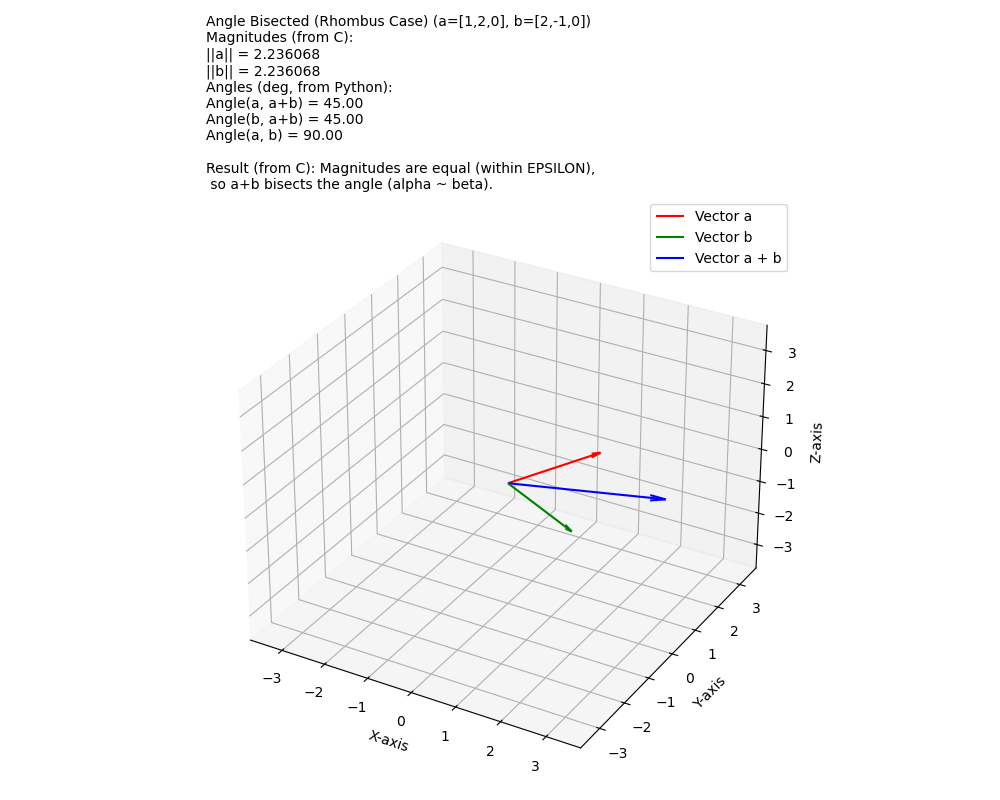
\includegraphics[width = 0.8\columnwidth]{figs/Figure_1.png}
					\caption*{}
					\label{}
				\end{figure}
			\end{center}
		\end{frame}
		
		
	\end{document}